\newpage
\chapter{Results}
\section{Empirical comparison of described models}\label{sec:results}
The models were tested on a set of job lists. Malapert's paper uses benchmark
job lists by \citet{daste1, daste2}. Since neither publication is
available online, I created my own set of randomized job lists for the purposes
of this paper, with $s_j, p_j \in [1, 20]$ and $d_j \in [1, 10n_j]$ where $n_j$ is
the number of jobs.\footnote{These instances will be updated to reflect the
feature distributions used in Daste et al.} Ten different sample job sets are
used per unique value of $n_j$. The times shown in figure \ref{fig:comp_times}
are averaged over those ten instances for each $n_j$.

The models were run on an i7 Q740 CPU in single-thread mode, with 8 GB RAM.
Solving was aborted after a time of 3600 seconds (1 hour).

The CP branch-and-bound model times out on most instances and is not shown here.
The CP model times out on one 12-job instance and gets progressively worse with
more jobs; similar to Malapert's original MIP model.
\begin{figure}
\centering

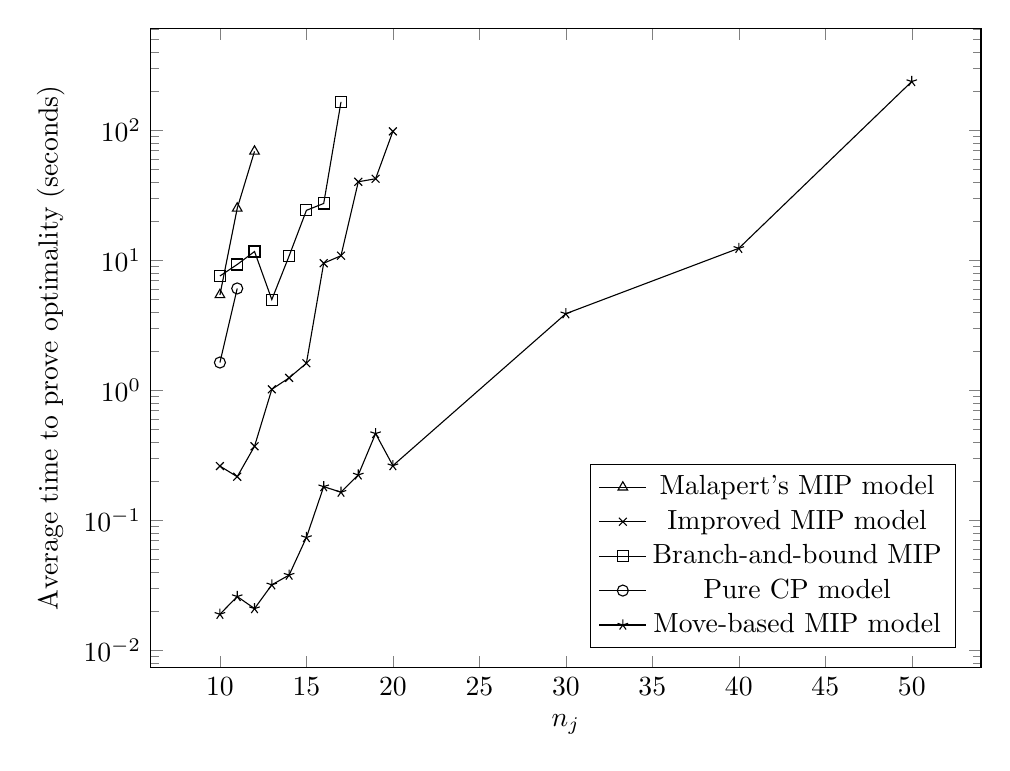
\begin{tikzpicture}
  \begin{semilogyaxis}[xlabel=$n_j$, ylabel=Average time to prove optimality (seconds), width=\textwidth,
  height=0.8\textwidth,legend pos=south east]
  \addplot[color=black, mark=triangle ] coordinates { % MIP model times
  (10, 5.441)
  (11, 25.18)
  (12, 69.05)
  };   \addlegendentry{Malapert's MIP model}

  \addplot[color=black, mark=x ] coordinates { % MIP model times
  (10, 0.262)
  (11, 0.217)
  (12, 0.372)
  (13, 1.02)
  (14, 1.25)
  (15, 1.62)
  (16, 9.52)
  (17, 10.88)
  (18, 40.3)
  (19, 42.5)
  (20, 98.415)
  };   \addlegendentry{Improved MIP model}

  \addplot[color=black, mark=square] coordinates {
(10, 7.59)
(11, 9.31)
(12, 11.72)
(13, 5)
(14, 10.83)
(15, 24.28)
(16, 27.44)
(17, 165.82)
  };
  \addlegendentry{Branch-and-bound MIP}
  \addplot[color=black, mark=o] coordinates {
(10, 1.64)
(11, 6.09)
};
  \addlegendentry{Pure CP model}
  \addplot[color=black, mark=star] coordinates {
(10, 0.019)
(11, 0.026)
(12, 0.021)
(13, 0.032)
(14, 0.038)
(15, 0.074)
(16, 0.182)
(17, 0.165)
(18, 0.224)
(19, 0.466)
(20, 0.264)
(30, 3.895)
(40, 12.403)
(50, 238)
};
  \addlegendentry{Move-based MIP model}
  \end{semilogyaxis}
\end{tikzpicture}

\caption{Comparison of CPU time used by different models to find an optimal
schedule and prove its optimality.}
\label{fig:comp_times}
\end{figure}




